\documentclass[letter,11pt]{article}
\usepackage{latexsym}
\usepackage{xcolor}
\usepackage{float}
\usepackage{amsthm}
\usepackage{esint}
\usepackage{amssymb}
\usepackage{wrapfig}
\usepackage{tabularx}
\usepackage{titlesec}
\usepackage{tikz}
\usepackage{geometry}
\usepackage{verbatim}
\usepackage{enumitem}
\usepackage{fancyhdr}
\usepackage{pgfornament}
\usepackage{multicol}
\usepackage{systeme}
\usepackage{graphicx}
\usepackage{mathtools}
%\usepackage{cfr-lm}
\usepackage{booktabs}
\usepackage{svg}
\usepackage[T1]{fontenc}
\usetikzlibrary{trees}
\setlength{\multicolsep}{0pt} 
\pagestyle{fancy}
%\fancyhf{} % clear all header and footer fields
\fancyhead{}\fancyfoot{}
\fancyhead[R]{\textbf{\thepage}}
\fancyhead[L]{Aiden M. Rosenberg, MMXXIII A.D. }
\addtolength{\headwidth}{3cm}

\usepackage{pgfplots}
\pgfplotsset{compat=1.17}
\usepgfplotslibrary{fillbetween}

\usepackage{pst-plot}
\usepgfplotslibrary{polar}



\renewcommand{\headrulewidth}{1pt}
\renewcommand{\footrulewidth}{0pt}
\geometry{left=1.5cm, top=2.5cm, right=1.5cm, bottom=2cm}

%\usepackage{draftwatermark}	
%\SetWatermarkColor[gray]{0.9}
%\SetWatermarkText{Private}
%\SetWatermarkScale{3}

\usepackage[most]{tcolorbox}
\tcbset{
	frame code={}
	center title,
	left=0pt,
	right=0pt,
	top=0pt,
	bottom=0pt,
	colback=gray!20,
	colframe=white,
	width=\dimexpr\textwidth\relax,
	enlarge left by=-2mm,
	boxsep=4pt,
	arc=0pt,outer arc=0pt,
}


\raggedright
\setlength{\tabcolsep}{0in}

% Sections formatting
\titleformat{\section}{
  \vspace{-4pt}\scshape\raggedright\large
}{}{0em}{}[\color{black}\titlerule \vspace{-7pt}]

\begin{document}

\thispagestyle{empty}

\fontfamily{cmr}\selectfont
%----------HEADING-----------------

\parbox{2.35cm}{%
	\includesvg[width=2.3cm]{logo.svg}
}
\parbox{0.3cm}{\hspace{0.3cm}}
\parbox{\dimexpr\linewidth-5cm\relax}{
	\setlength{\tabcolsep}{0.5em}
	\def\arraystretch{1.25}
	\begin{tabular}{@{}llll@{}}
		\toprule
		\multicolumn{4}{c}
		{\hspace{-0.5em}\textbf{Assignment}: Worksheet \#7 (16.3, 16.4)} \\ \midrule
		\textbf{Name:}   & D. Aiden M. Rosenberg & \textbf{Professor:} & Dr. Alan v. Herrmann Ph.D \\
		\textbf{Course:} & Calculus III          & \textbf{Date:}      & October 28th, 2023 A.D.   \\ \bottomrule
	\end{tabular}
}
\vspace{1cm}

\section*{Section 16.3}
Evaluate $\displaystyle \int_{-2}^{0}\int_{-\sqrt{4-y^2}}^{\sqrt{4-y^2}} x^2 \,dx\,dy$.
\begin{figure}[h]
	\centering
	\begin{tikzpicture}[scale = 0.75]
		\begin{axis}[
				domain=-2:2,           % Set the x-axis domain
				samples=400,               % Number of samples to plot
				axis lines=middle,         % Position the axes
				xlabel=$x$,                % x-axis label
				ylabel=$y$, 
				xmin=-3,
				xmax=3,
				ymin=-3,
				ymax=3,% y-axis label
			]
						        
			% Plot the functions and define name paths
			\addplot[black, thick, name path=A] {sqrt(4-x^2)};
			\addplot[black, thick, name path=B] {-sqrt(4-x^2)};
						        
			% Define name path for the x-axis
			\path[name path=xaxis] (axis cs:-2.5,0) -- (axis cs:2.5,0);
						        
			% Shade the area between the x-axis and curve B
			\addplot[violet, opacity=0.5] fill between[of=xaxis and B];
		\end{axis}
	\end{tikzpicture}
	\caption{Region of integration}
\end{figure}

\begin{align*}
	\int_{-2}^{0}\int_{-\sqrt{4-y^2}}^{\sqrt{4-y^2}} x^2 \,dx\,dy & =                                                                                \\
	                                                              & = \int_{-\pi}^{0}\int_{0}^{2}\left(r\cos\theta\right)^{2}r dr\,d\theta           \\
	                                                              & = \int_{-\pi}^{0}\int_{0}^{2}r^{3}\cos^{2}\theta\ dr\, d\theta                   \\
	                                                              & = \int_{0}^{\pi} \left[\frac{r^4}{4}\right]_{r=0}^{r=2}\cos^{2}\theta \, d\theta \\
	                                                              & = 4\int_{-\pi}^{0}\cos^{2}\theta d\theta                                         \\
	                                                              & = 4\int_{0}^{\pi} \cos^2(u) \, du                                                \\
	                                                              & = 4\int_{0}^{\pi} \frac{(1+\cos(2x)}{2} \, d\theta                               \\
	                                                              & = 4\left[\frac{1}{2}\theta + \frac{1}{4}\sin(2\theta)\right]_{-\pi}^{0}          \\
	                                                              & = 4 \cdot \frac{\pi}{2}                                                          \\
	                                                              & = \boxed{2\pi}                                                                   
\end{align*}
\newpage
\section*{Section 16.3 cont.}
Consider region $D$ inside $r = 4\sin\theta$ and outside $r = 2$.
\begin{figure}[h]
	\centering
	\begin{tikzpicture}[scale = 0.75]
		\begin{polaraxis}[
				xmin=0,
				xmax=360,
				xtick distance=deg(pi/4),
				xtick={0, deg((pi)/4), deg((pi)/2), deg((3*pi)/4), deg(pi), deg((3*pi)/2)},
				xticklabels={0, $\frac{\pi}{4}$, $\frac{\pi}{2}$, $\frac{3\pi}{4}$, $\pi$, $\frac{3\pi}{2}$},
				ymajorgrids=true,
				grid=both,
			]
						
			% Plot the first polar curve r = 4sin(theta)
			\addplot+[mark=none,smooth,blue, thick, domain=0:360,samples=360,name path=curve1] {4*sin(x)};
			\addlegendentry{$r = 4\sin\theta$}
						
			% Plot the second polar curve r = 2
			\addplot+[mark=none,smooth,black,thick,domain=0:360,samples=360,name path=curve2] {2};
			\addlegendentry{$r = 2$}
						
			\addplot[fill=violet, opacity=0.5, domain=0:180, samples=360] {4*sin(x)};
			\addplot[fill=white, opacity=0.5, domain=-30:30, samples=360] {4*sin(x)};
			\addplot[fill=white, opacity=0.5, domain=30:150, samples=360] {2};
						
			\draw (90, 3) node {$D$};
		\end{polaraxis}
	\end{tikzpicture}
		
	\caption{Region of integration}
\end{figure}
\begin{enumerate}[label = \roman*.]
	\item Graph and shade region $D$.
	      \begin{enumerate}
	      	\item Reference Figure 2
	      \end{enumerate}
	\item Find the area of this region.
	      \begin{align*}
	      	A & = \int_{\frac{\pi}{6}}^{\frac{5\pi}{6}}\int_{2}^{4\sin\theta}\ r \, dr \,d\theta                                                                                           \\
	      	  & = \int_{\frac{\pi}{6}}^{\frac{5\pi}{6}}\left[\frac{r^2}{2}\right]_{r=2}^{r=4\sin\theta}\,d\theta                                                                           \\
	      	  & = \frac{1}{2}\int_{\frac{\pi}{6}}^{\frac{5\pi}{6}} \left(\left(4\sin\theta\right)^{2}-\left(2^{2}\right)\right) \, d\theta                                                 \\
	      	  & = \frac{1}{2}\int_{\frac{\pi}{6}}^{\frac{5\pi}{6}}\ \left(16\sin^{2}\theta-4\right)\, d\theta                                                                              \\
	      	  & = 2\int_{\frac{\pi}{6}}^{\frac{5\pi}{6}}\ \left(4\sin^{2}\theta-1\right) \, d\theta                                                                                        \\ 
	      	  & = 8\int_{\frac{\pi}{6}}^{\frac{5\pi}{6}}\ \left(\sin^{2}\theta\right)d\theta\ -\ 2\int_{\frac{\pi}{6}}^{\frac{5\pi}{6}}\,d\theta                                           \\
	      	  & = 8\int_{\frac{\pi}{6}}^{\frac{5\pi}{6}}\ \left(\frac{\theta - \sin 2\theta}{2}\right) \, d\theta\ -\frac{4\pi}{3}                                                         \\
	      	  & = 4\left[\theta - \sin(2\theta)\right]_{\frac{\pi}{6}}^{\frac{5\pi}{6}} -\frac{4\pi}{3}                                                                                    \\
	      	  & = 4\left(\left(\frac{5\pi}{6}-\frac{1}{2}\sin\left(\frac{5\pi}{3}\right)\right)-\left(\frac{\pi}{6}-\frac{1}{2}\sin\left(\frac{\pi}{3}\right)\right)\right)-\frac{4\pi}{3} \\
	      	  & = \boxed{\frac{4\pi}{3}+2\sqrt{3}}                                                                                                                                         
	      \end{align*}
\end{enumerate}

\section*{Section 16.4}
Consider the solid below $f(x,y)=24-3x-4y$ and above region $R = \{(x, y)| 0 \leq x \leq 3, 0 \leq y \leq 2\}$
\begin{figure}[h]
	\centering
	\begin{tikzpicture}
		\begin{axis}[
				view={120}{30},
				axis lines=middle,
				xlabel={$x$},
				ylabel={$y$},
				zlabel={$z$},
				xlabel style={below left},
				ylabel style={below left},
				zlabel style={above},
				xmin=-2, xmax=10,
				ymin=-2, ymax=8,
				zmin=-2, zmax=30,
				tick style={ultra thick},
				xtick={0,8},
				ytick={0,6},
				ztick={0,24},
			]
			
			% Plot the plane
			\addplot3[surf, opacity=0.5, domain=0:8, domain y=0:6] {24 - 3*x - 4*y};
		\end{axis}
	\end{tikzpicture}
        \caption{Graph of $f(x,y)$}
\end{figure}
\begin{enumerate}[label = \roman*.]
	\item Sketch a well-labeled graph of the solid.
            \begin{enumerate}
                \item Reference Figure 3
            \end{enumerate}
	\item Set-up a double integral to find the volume of this solid. (Do not evaluate).
        $$\text{Volume} = \boxed{\int_{0}^{3}\int_{0}^{2} \left(24-3x-4y\right)\, dy\,dx}$$
	\item Set-up and evaluate a triple integral to find the volume of this solid. (Evaluate this integral).
        \begin{align*}
            \text{Volume} &= \iiint_{R} 1 \, d V \\
            &= \int_{0}^{3}\int_{0}^{2} \int_{0}^{24-3x-4y} 1 \, dz\, dy\, dx\\
            &= \int_{0}^{3}\int_{0}^{2} [x]_{0}^{24-3x-4y} \, dy\, dx\\
            &= \int_{0}^{3}\int_{0}^{2} \left(24-3x-4y\right)\, dy\,dx\\
            &= \int_{0}^{3} \left[24y-3xy-2y^2\right]_{y=0}^{y=2} \,dx\\
            &= \int_{0}^{3}\left(40-6x\right) \, dx\\
            &= \left[40x-3x^2\right]_{x=0}^{x=3} \\
            &= 120- 27 = \boxed{93}
        \end{align*}

\end{enumerate}
\newpage
\section*{Section 16.4 cont.}
Consider solid $E$ bounded above by $z = 12-y$, below by $z = 0$, and laterally by $y = 3x^2$.

\begin{enumerate}[label = \roman*.]
\begin{figure}[h]
             \centering
             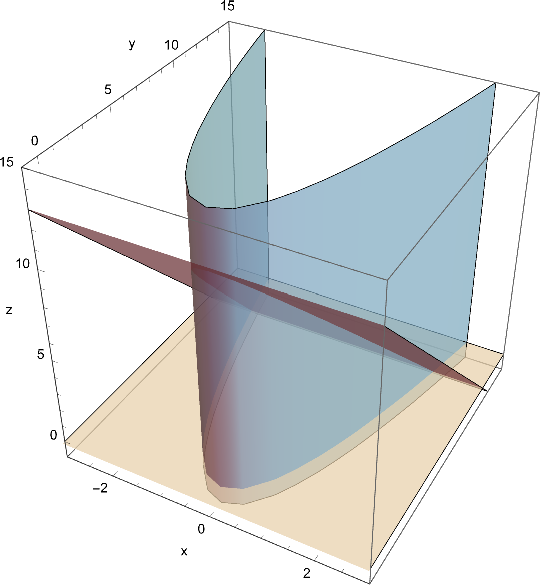
\includegraphics[width = 2in]{Graph1.pdf}
             \caption{Graph of solid $E$}
         \end{figure}
	\item Sketch a well-labeled graph of solid $E$.
         \begin{enumerate}[label = \roman*.]
             \item Reference Figure 4 \footnote{I couldn't determine how to create a \LaTeXe representation for this graph, so I opted to utilize Wolfram Mathematica software instead.}
         \end{enumerate}
	\item \underline{Set-up} a triple integral to find the volume of solid $E$ using order $dV = dz\, d, dx$. (Do not evaluate).
 \begin{enumerate}[label = \roman*.]
    \item When $z=0\Longrightarrow y= 12 \Longrightarrow x= \pm 2$.
    \item $x\in[-2,2]$, $y\in[0,12]$, \& $z\in[0,12]$
 \end{enumerate}
 $$\boxed{\int_{-2}^{2}\int_{3x^2}^{12}\int_{0}^{12-y} \, dz\,dy\,dx}$$
	      	      
\end{enumerate}
\end{document}
